\section{Software architecture views}
asdf
\subsection{Subsystem decomposition}
asdf
\newpage
\subsection{Hardware/software mapping}
In this section the hardware/software mapping Tygron uses will be explained, as well as the way our agent will be connected to this.

\subsubsection{Tygron}
Tygron has its own server, from which it communicates with all other entities. For each group of users, there is a seperate server which contains their world and on which those users can work. The general Tygron server knows these other servers and will redirect the user to the particular server. So, when a customer wants to connect to Tygron, it will first connect to this general server. Also, this general server has contact with other servers which are not connected to Tygron. For example, when a customer wants to build a part of a city to play on, the general server will connect to some other servers that give information about this place, like where the buildings are and what the use of those buildings is. 

\subsubsection{Our project}
In our project we have our own server with all TU Delft students. But there is another thing that needs to be different: the way we connect to that server. Since we don't use humans, but agents to play the game, those agents need to connect in some way to the server. To do so we have a connector between our instance and the server. This connector will use the goal code we wrote and will translate this into actions in the game. This way our agent can play the game. The picture in Persistent data management illustrates this.

\newpage
\subsection{Persistent data management}
The data management for our project envelops multiple things. We have a part where the data for the game is stored and the data we need for running the agent. The first part is done by Tygron. When a new project is created it is stored in the Tygron database to which the clients can connect via the Tygron server. Any changes made in a session are then updated to the database, which are visible to all the other clients. Figure \ref{fig:tygron1} shows the diagram of the Tygron Engine connected to the database and the GOAL agent.

\begin{figure}[h!]
  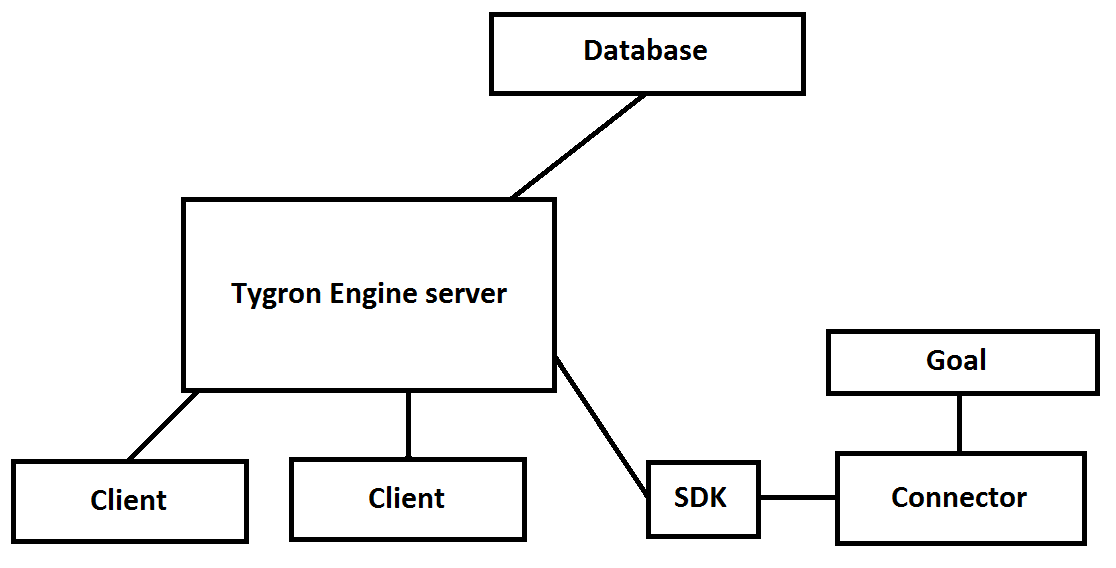
\includegraphics[width=\linewidth]{Tygrondatabase.png}
  \caption{Diagram of the Tygron Engine connected to the database and the GOAL agent.}
  \label{fig:tygron1}
\end{figure}

In GOAL the data the agent uses is stored in multiple databases. The agent has a knowledge base which is the same for every environment that he might find himself in. This data is simply stored as GOAL code in the agent his GOAL files. The rest of the data that the agent uses is dynamic and his state is updated constantly according to the situation that the agent is currently in. Our agent maintains two different databases of facts. One database called the goal base consists of things the agent wants to achieve. The other database is called the belief base and consists of facts that the agent believes are true (now).  Figure \ref{fig:agentstate1} shows how the databases of the agent are updated.

\begin{figure}[h!]
  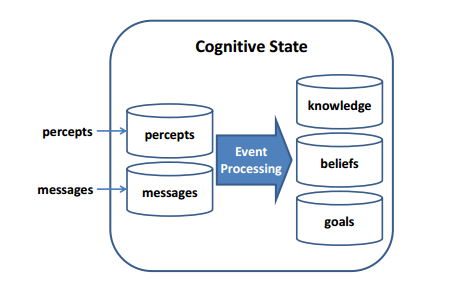
\includegraphics[width=\linewidth]{agentstate.png}
  \caption{Updating the agent's database.}
  \label{fig:agentstate1}
\end{figure}

\newpage
\subsection{Concurrency}
Each group in the Virtual Humans for Serious Gaming context project will develop a cognitive agent, so there will be 5 roles and therefore multiple agents. An agent itself does not make use of concurrency, but all the agents together will run parallel and are running in 1 environment. When there are multiple agents running, there is concurrency. A crucial thing to find solutions for city design and development projects in a game is communication between the agents. The agents have to be able to communicate and find a solution together that fulfil the goals of the agents as much as possible.




